\documentclass[border=10pt,tikz]{standalone}
\usepackage{amsmath}
\usetikzlibrary{angles,quotes}
\begin{document}
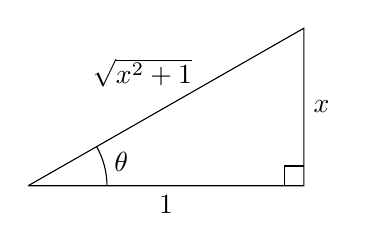
\begin{tikzpicture}[
  my angle/.style={
    every pic quotes/.append style={text=black},
    draw=black,
    angle radius=1cm,
  }]
  \coordinate (C) at (-2,-1);
  \coordinate (A) at (1.5,-1);
  \coordinate (B) at (1.5,1);
  % \coordinate [label=left:$C$] (C) at (-1.5,-1);
  % \coordinate [label=right:$A$] (A) at (1.5,-1);
  % \coordinate [label=above:$B$] (B) at (1.5,1);
  \draw (C) -- node[label={[shift={(-3mm,0mm)}]$\sqrt{x^2+1}$}] {} (B) 
-- node[right] {$x$} (A)
-- node[below] {$1$} (C);
  \draw (A) +(-.25,0) |- +(0,.25);
  % \pic [my angle, "$\tfrac x2$"] {angle=A--C--B};
  \pic ["$\theta$" shift={(6mm, 1.5mm)}, draw, angle radius=1cm] {angle=A--C--B};
  % \pic [my angle, "$\beta$"] {angle=C--B--A};
\end{tikzpicture}
\end{document}